\documentclass[12pt,letterpaper]{ctexart}
\usepackage{fullpage}
\usepackage[top=2cm, bottom=4.5cm, left=2.5cm, right=2.5cm]{geometry}
\usepackage{amsmath,amsthm,amsfonts,amssymb,amscd}
\usepackage{lastpage}
\usepackage{enumerate}
\usepackage[binary-units=true]{siunitx}
\usepackage{fancyhdr}
\usepackage{mathrsfs}
\usepackage{xcolor}
\usepackage{graphicx} %插入图片的宏包
\usepackage{float} %设置图片浮动位置的宏包
\usepackage{subfigure} %插入多图时用子图显示的宏包
\usepackage{listings}
\usepackage{afterpage}
\usepackage{hyperref}
\hypersetup{
    colorlinks=true,
    linkcolor=blue,
    filecolor=magenta,
    urlcolor=cyan,
}

\newcommand\blankpage{%
  \null
  \thispagestyle{empty}%
  \addtocounter{page}{-1}%
  \newpage
}


\hypersetup{%
  colorlinks=true,
  linkcolor=blue,
  linkbordercolor={0 0 1}
}

\renewcommand\lstlistingname{Algorithm}
\renewcommand\lstlistlistingname{Algorithms}
\def\lstlistingautorefname{Alg.}

\lstdefinestyle{Python}{
    language        = Python,
    frame           = lines,
    basicstyle      = \footnotesize,
    keywordstyle    = \color{blue},
    stringstyle     = \color{green},
    commentstyle    = \color{red}\ttfamily
}

\setlength{\parindent}{0.0in}
\setlength{\parskip}{0.05in}

% Edit these as appropriate
\newcommand\course{CS305}
\newcommand\hwnumber{6}                  % <-- homework number
\newcommand\NetIDa{11711918}           % <-- NetID of person #1
\newcommand\NetIDb{吴烨昌}           % <-- NetID of person #2 (Comment this line out for problem sets)

\pagestyle{fancyplain}
\headheight 35pt
\lhead{\NetIDa}
\lhead{\NetIDa\\\NetIDb}                 % <-- Comment this line out for problem sets (make sure you are person #1)
\chead{\textbf{\Large Assignment \hwnumber}}
\rhead{\course \\ \today}
\lfoot{}
\cfoot{}
\rfoot{\small\thepage}
\headsep 1.5em

\begin{document}

\section*{Problem 1}

{\bf Description}

Open ``Network'' view in ``developer tools'' of browse(such as chrome) to observe
\begin{itemize}
  \item Is there any `mpd' files, What’s its name, what is the description of `mpd' in mime
  \item Is there any `m4s' files, what’s its related rate, will the files’ `rate' change along with the changing of network condition(especially the bandwidth)
\end{itemize}


{\bf Solution}

Open url \href{http://reference.dashif.org/dash.js/nightly/samples/dash-if-reference-player}{http://reference.dashif.org/dash.js/nightly/samples/dash-if-reference-player},
and watch ``Network'' tab in ``DevTools''.

\begin{itemize}
  \item There is only 1 ``mpd'' file, named ``bbb\_30fps.mpd'', whose MimeType is ``Application\/dash-xml''
  \begin{figure}[H]
    \centering
    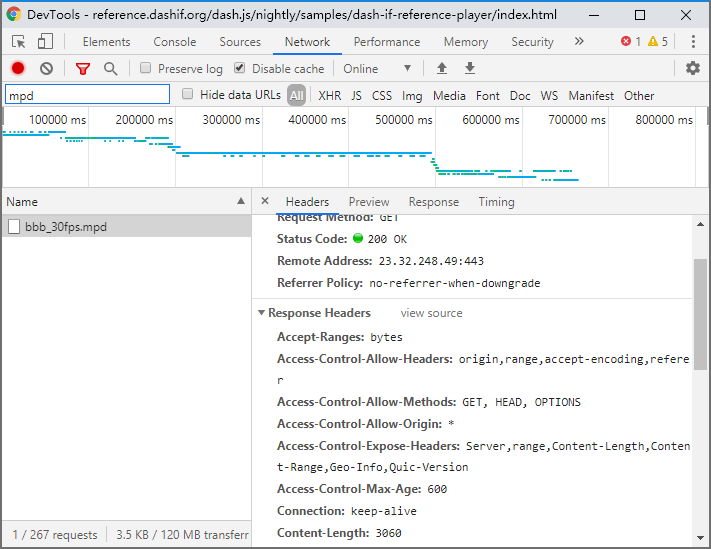
\includegraphics[width=0.7\linewidth,natwidth=610,natheight=550]{assets/6.1_mpd.png}
    \caption{mpd request in Network}
    \label{fig:mpd}
  \end{figure}

  \item There is no ``m4s'' file but many ``m4a'' and ``m4v'' files. The number of them are increasing with time.
  The files' related rate is the bitrate in the filename. The files’ `rate' change along with the changing of network condition, the bigger bandwidth is, the greater the file's bitrate is.

  \begin{figure}[H]
    \centering
    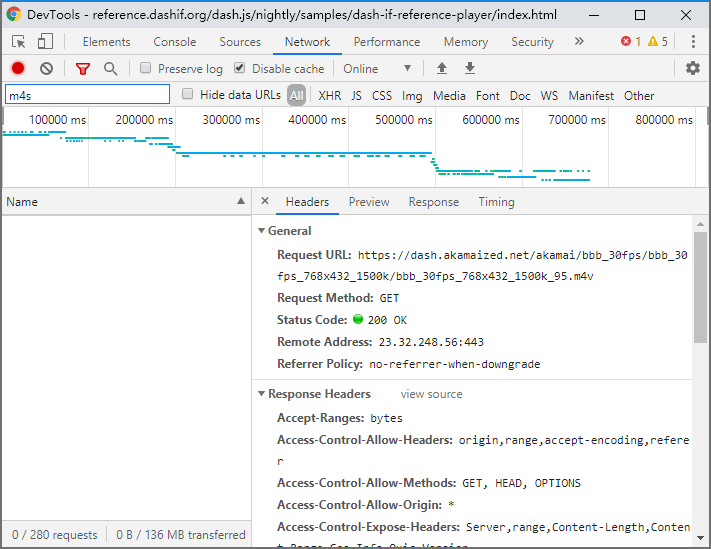
\includegraphics[width=0.7\linewidth,natwidth=610,natheight=642]{assets/6.1_m4s.png}
    \caption{m4s request in Network}
    \label{fig:m4s}
  \end{figure}

  \begin{figure}[H]
    \centering
    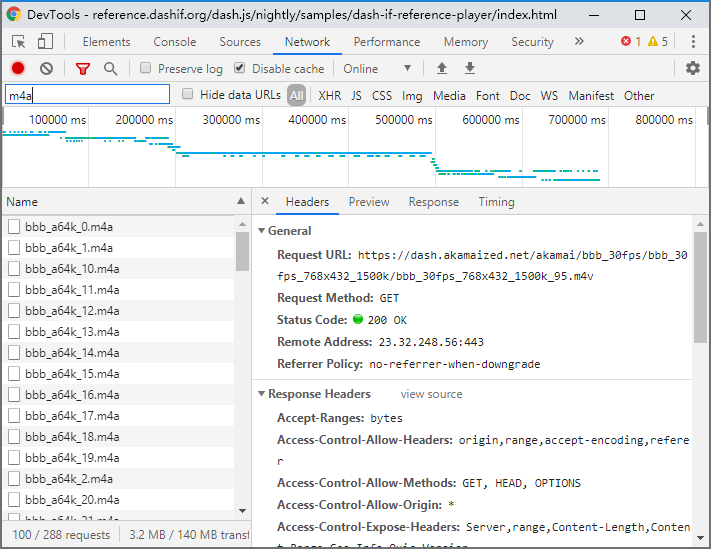
\includegraphics[width=0.7\linewidth,natwidth=610,natheight=642]{assets/6.1_m4a.png}
    \caption{m4a request in Network}
    \label{fig:m4a}
  \end{figure}

  \begin{figure}[H]
    \centering
    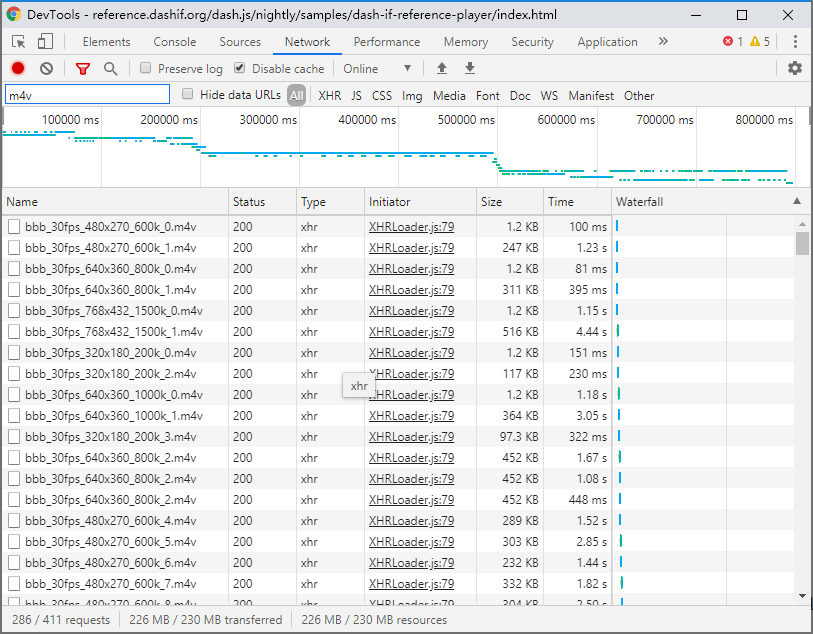
\includegraphics[width=0.65\linewidth,natwidth=650,natheight=642]{assets/6.1_m4v.png}
    \caption{m4v request in Network}
    \label{fig:m4v}
  \end{figure}
\end{itemize}

\end{document}
